\section{Ejercicio 3}

\subsection{Descripci\'on}
El ejercio 3 consiste en completar una fracci\'on de la simulaci\'on de los avances de los frentes magn\'eticos
en interfaces de medios desordenados. Para eso se gener\'o un modelo basado en mec\'anica cl\'asica, usando
\textit{splines} para trazar las curvas de las particulas y \textit{springs} para delimitar el frente.

El c\'odigo fue hecho usando la librer\'ia \texttt{thrust} para poderlo correr en CPU y GPU indistintamente.
Tambien se utiliz\'o un random number generator especial, basado en contadores, para no tener que almacenar las posiciones 
hist\'oricas de cada particula. Esto hace manejable los tama\~nos de de mem\'oria de modo que entren en las placas
aceleradoras GPGPU. 

\subsection{TODOs}
El primer \texttt{TODO} era relacionado al RNG. Este TODO se\~nalaba que habia un error con respecto al
uso del RNG en el caso del ruido t\'ermico. Habia que entender como funcionaba un counter-based RNG para
poder entender cual era el error ahi. El problema radicaba en como obtener n\'umeros aleatorios no correlacionados
pero que sigan siendo reproducibles de la misma manera que los usados para el desorden del medio. 
Los counter-based RNG toman dos parametros, un counter y una key, y devuelven un numero aleatorio. Llamar
con los mismos parametros al RNG siempre devuelve el mismo n\'umero. Esto indica que para obtener 
el siguiente valor de la secuencia random, habr\'ia que modificar el counter. Sin embargo, quisieramos
obtener valores aleatorios tambien para el otro ruido, y debieramos seedearlos distinto para que no
haya ninguna correlaci\'on entre ellos. Para eso, habria que variar la key, y setearla al seed correspondiente.

Los CBRNG usados aca toman como key el valor del thread donde estan haciendo el computo, y como counter 
la uni\'on de un seed de cada fuente de numeros aleatorios con el $u$ usado, donde $u$ es la posici\'on del mon\'omero
actual. De esta manera los valores random son reproducibles hacia atras y hacia adelante.

Dicho todo esto, el FIXME consistia en entender la teoria de los CBRNG y ver que el uso que se le estaba dando
no generaba valores aleatorios diferentes, sino que los podia repetir. La soluci\'on consistia en hacer que el ruido
t\'ermico dependiera del tiempo de la simulaci\'on, es decir, que no pueda volver para atras el ruido termino.
Esto se hacia duplicando el mecanismo usado anteriormente y cambiando el seed al seed2 y el $u$ por el $t$ de la simulaci\'on.


El segundo \texttt{TODO} se referia al c\'alculo de dos propiedades de la interfaz, la velocidad y la posicion del centro de masas.
Recordemos que la velocidad se calcula como $V = \frac{\Delta x}{\Delta t}$ y el centro de masas (dadas las hipotesis del problema)
se calcula como $P = \frac{\Sigma_i P_i}{L}$. Para calcular el centro de masas, debemos obtener la posicion de cada uno de los
puntos y promediarla. Como el problema son $L$ puntos equiespaciados en la coordenada $y$, tomamos solamente los valores 
de X para obtener el centro de masas. Esto se traduce en un c\'odigo de thrust de reduce asi: \\
\texttt{ REAL center\_of\_mass = reduce(u\_it0, u\_it1, 0.0) / L;}\\
Esto hace una suma de todos las posiciones en X de las particulas y las promedia al dividirlas por L (fuera de la placa).

Para obtener la velocidad del centro de masas, deberiamos ver cuanto cambio su posici\'on con respecto del tiempo, $\Delta t$
Para eso, antes de la iteraci\'on de euler inmediata anterior al calculo de propiedades, nos guardamos todas las posiciones
de las particulas (podria reducirse el uso de memoria haciendo un reduce ahi mismo).
Luego el c\'odigo relevante es:\\
\newcommand*\justify{%
  \fontdimen2\font=0.4em% interword space
  \fontdimen3\font=0.2em% interword stretch
  \fontdimen4\font=0.1em% interword shrink
  \fontdimen7\font=0.1em% extra space
  \hyphenchar\font=`\-% allowing hyphenation
}
\texttt{\justify{REAL velocity =  (( (L*center\_of\_mass) - reduce(u\_old.begin()+1,u\_old.end()-1,0.0) 
                                 ) / L  
                                 ) /Dt;  
                             }}\\
Con esto obtenemos el delta posicion arriba, y primero lo dividimos por la cantidad de elementos para obtener el promedio de los
delta por punto, y luego lo dividimos otra vez por el delta tiempo para obtener la tasa de variacion de la posicion en funcion
de un step de tiempo, es decir, la derivada de la posici\'on en funci\'on del tiempo, que es la velocidad del centro de masas.


 % \begin{figure}[H]
 % \begin {center}
 % 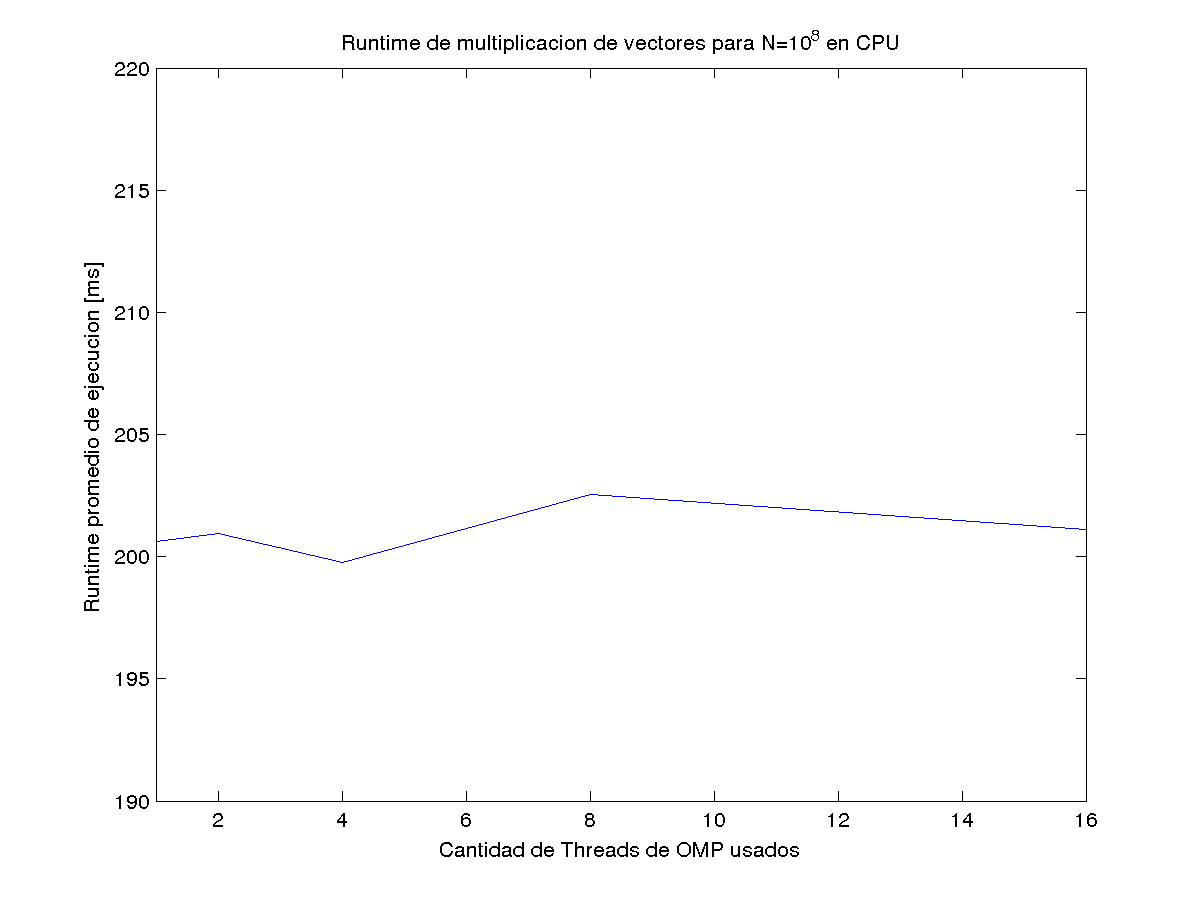
\includegraphics[width=\hrwidth]{plots/ej1omp.png}
 % \end {center}
 % \caption{Runtime del ej1 en Thrust con OMP, en funcion de la cantidad de threads, para una longitud de vectores $L=10^8$}
 % \label{fig:ej1OMP}
 % \end{figure}

% \begin{table}
 %    \begin{tabular}{l|l}
 %       \textbf{M\'etodo} & \textbf{ Runtime [ms] }\\ \hline
 %   1 OMP Thread         & 200.598      \\
 %   2 OMP Thread          & 200.963      \\
 %   4 OMP Thread          & 199.766      \\
 %   8 OMP Thread  & 202.534      \\
 %   16 OMP Thread & 201.127      \\
 %       CUDA M2090 & 11.035 
 %   \end{tabular}
%\end{table}



 Como se puede ver en el gr\'afico y la tabla de la figura \ref{fig:ej1OMP}, casi no varian los runtimes a pesar de tener
 muchos threads. Esto se debe a que el costo de generar y spawnear threads nuevos es tan alto que el procesador
 deberia hacer m\'as c\'alculo por core en vez de paralelizar m\'as el problema. Esto es un claro ejemplo
 de una tarea que es demasiado chica para threadear, e incluso con un problema relativamente grande de $10^8$ 
 elementos, no vale la pena paralelizarlo con CPU.

 Comparado contra la placa Nvidia con CUDA, podemos apreciar la diferencia de velocidad notablemente. Esto igual no toma
 en cuenta el tiempo de transferencia de memoria, por lo cual puede llegar a ser engañoso a veces el tiempo de runtime
 en las comparaciones CPU/GPU.
